\documentclass[10pt,twocolumn,letterpaper]{article}

\usepackage{cvpr}
\usepackage{times}
\usepackage{epsfig}
\usepackage{graphicx}
\usepackage{amsmath}
\usepackage{amssymb}

\newenvironment{tightenumerate}{
\begin{enumerate}
  \setlength{\itemsep}{1pt}
  \setlength{\parskip}{0pt}
  \setlength{\parsep}{0pt}
}{\end{enumerate}
}

% this makes list spacing much better.
\newenvironment{tightitemize}{
\begin{itemize}
  \setlength{\itemsep}{1pt}
  \setlength{\parskip}{0pt}
  \setlength{\parsep}{0pt}
}{\end{itemize}
}

\cvprfinalcopy % *** Uncomment this line for the final submission

\def\cvprPaperID{****} % *** Enter the CVPR Paper ID here
\def\httilde{\mbox{\tt\raisebox{-.5ex}{\symbol{126}}}}

% Pages are numbered in submission mode, and unnumbered in camera-ready
\ifcvprfinal\pagestyle{empty}\fi

\begin{document}

\title{Segmentation Using Attributes}

\author{Aibo Tian\\
%Institution1\\
%Institution1 address\\
{\tt\small atian@cs.utexas.edu}
% For a paper whose authors are all at the same institution,
% omit the following lines up until the closing ``}''.
% Additional authors and addresses can be added with ``\and'',
% just like the second author.
% To save space, use either the email address or home page, not both
\and
John Edwards\\
%Institution2\\
%First line of institution2 address\\
{\tt\small edwardsj@cs.utexas.edu}
}

\maketitle
\thispagestyle{empty}

%-------------------------------------------------------------------------------
% abstract
%-------------------------------------------------------------------------------
\begin{abstract}
Attributes have been shown to be effective in assisting object detection and
classification, and they provide means to also incorporate semantic
information available to and provided by humans.  On another front, the
combination of segmentation and object classification has been shown to
improve both segmentation and classification.  We present a method of incorporating
attributes into segmentation using a hierarchical methodology.
That is, using attributes as features, we discover attributes of regions
at all levels of a hierarchical segmentation, 
incorporate hierarchical confidences in determining a confidence that
a given region is part of a given object, and segment the image using
these confidences.  We also present results from experiments run using
this method.
\end{abstract}

%-------------------------------------------------------------------------------
% introduction
%-------------------------------------------------------------------------------
\section{Introduction}
Very recent work on using attributes as features \cite{farhadi09, lampert09}
has shown that attributes are an effective way of communicating information
about an object in an image.  Attributes are, in essence, semantic high-level
features.  The attributes of an image are learned using low-level features,
and once learned, they can be used in object detection and also in describing
objects in an image that are unknown.

Image segmentation is a very different field of research and has a very different
goal - that of finding very accurate boundaries of objects in an image.

Our work focuses on leveraging attributes to produce accurate segmentations.
The idea is to find image regions with salient attribute distributions.  If
these regions can be combined together to for larger regions with attribute 
distributions matching some object's canonical distribution then one can
declare the combined region an accurate segmentation for that object.

In practice, however, the testing of all combinations of regions to find 
objects is intractable.  We use two approximatory algorithms operating on
a segmentation hierarchy to determine salient regions.  Both are subtractive
algorithms, which first predict attributes on the entire region and then
proceed by observing the effects of removing different regions during
a top-down traversal of the tree.  The benefit of using these methods are
that large regions that clearly don't contribute to attribute saliency
can be pruned from the tree early in the traversal.  This approach avoids
the combinatoric complexity of a full search and, even more, prunes many
regions from the segmentation tree before they even are searched, bringing
the computational complexity, in practice, to roughly $O(n)$ where $n$ is
the number of leaves in the segmentation tree.

While we focus on segmentation of known objects, we anticipate an application
that takes more advantage of attributes: that of segmenting \emph{unknown}
objects from an image that exhibit salient but unrecognized attribute
distributions.  This type of application brings out some of the true power of
attributes, that of assigning semantic meaning to unknown, segmented objects.

This paper is organized as follows: we first discuss related work (\S \ref{sec:related_work})
and then present the algorithm in detail (\S \ref{sec:technical}).  We then discuss results from
a small-scale experiment on images from the pascal 2008 dataset (\S \ref{sec:results}), after which we draw
conclusions and discuss future directions (\S \ref{sec:conclusions}).

%-------------------------------------------------------------------------------
% related work
%-------------------------------------------------------------------------------
\section{Related work}
\label{sec:related_work}
A significant amount of recent work has been done in the area of using
attributes as high-level features for image classification and object
description \cite{farhadi09, lampert09, kumar09}.  
Another area of computer vision, that of segmentation,
has seen a resurgence of popularity as methods to incorporate top-down
information into segmentation have been shown to be highly effective
\cite{borenstein04, pantofaru, gu09, russell06, malisiewicz, leibe04, hoiem05, shotton06}.  
We propose to leverage research done in both of these areas -- attributes
and top-down/bottom-up segmentation -- to produce a combined approach.

Farhadi et al
\cite{farhadi09} use attributes as high-level features for object classification. They
can also describe an image using its attributes alone.
Lampert et al \cite{lampert09}
use the attributes as a intermediate layer between the low-level
features and object classes. Based on this layer, they can predict
disjoint classes that are not seen in the training set.  Both of these
approaches are geared toward object detection and classification.  While
our method goes further, incorporating segmentation, we will be using
the ideas and algorithms in \cite{farhadi09} for assignments of 
attributes to different segmented regions.

Object classification can give some top-down high-level information
for segmentation. On the other hand, segmentation can provide
image-based coherence information for classification. To deal with
the problem that the bottom-up single segmentation is not accurate,
more and more algorithms are based on multiple segmentations. Gu et
al \cite{gu09} uses the hierarchical segmentation algorithm to
generate multiple segments, and detect different parts of objects in
each segment. The final objects are voted for by the various parts.
We will initially be using the same segmentation algorithm used in
this paper, but without discarding the hierarchy.
Russell et al \cite{russell06} detect the whole object in each of
the multiple segment, by assuming that most objects get segmented
correctly at least once during the multiple segmentation. Our approach
will be far less aggressive in that we will use object classes and 
features (attributes in our case) that are known \emph{a priori}.
Pantofaru et
al \cite{pantofaru} use three different segmentation algorithms to
generate the multiple segments. After detecting objects in each
segment, they merge the intersected segments as final results. In
our method, we use common knowledge of distribution of attributes to
merge segments.
Borenstein et al \cite{borenstein04} proposed a method of combining top-down
and bottom-up information to generate a high-quality segmentation.  Their
approach to the top-down is to use exemplar image fragments and match them
to the image and then refining the top-down segmentation using their
segmentation hierarchy.  Our approach is very similar to this in spirit.
While our initial estimate of segmentation is from the bottom-up (while
theirs is from the top-down) we will use the hierarchical information
from the segmentation to boost confidences of segmentation at the lowest
level, similar to what they do.

Another interesting work is that of Gould et al \cite{gould08}.  They use
superpixels for an initial segmentation, build a CRF that includes a
relative location feature in the energy function and minimizes the CRF
for a final segmentation.  The relative location feature is determined
using prior location probability maps.  Our approach is similar to this
as well, in that we will also incorporate relative location information,
although ours will use attributes' relative locations rather than object
classes.  We will also use a CRF for the final segmentation, but will
use a min-cut solution since our labels are binary.
Kumar et al \cite{kumar05} incorporate shape structure into the segmentation by
adding a latent shape parameter to the CRF.  This seems like it would be
a useful addition to our system but make the scope too large.

%-------------------------------------------------------------------------------
% technical approach
%-------------------------------------------------------------------------------
\section{Technical approach}
\label{sec:technical}
Our approach begins with building a segmentation tree.  We use the segmentation
approach of \cite{arbelaez09} (in fact, we use their code).  This is a hierarchical
segmentation approach which first detects contours using the \emph{gPb} detector
\cite{maire08}.  Once the contours are detected, regions are discovered using a
watershed algorithm after which an Ultrametric Contour Map (UCM) is constructed,
which defines the region hierarchy.

The top node of this hierarchy is the image itself.  Our algorithm first predicts
attributes on the image.  Our attributes are trained using images from the pascal 
2008 dataset using the same annotations used in \cite{farhadi09}.  We trained using
an SVM with linear kernel.

TO TALK ABOUT:
? Discovered that our implementation learns largely on the object and not truly
on the different attributes.

We will assume that we know that an object is present in the image, as is done in \cite{borenstein04}, as opposed to no knowledge, as in \cite{shotton06}.  So we will have to use tagged examples.

The labeling will be binary - imageground and background, as opposed to multi-label results.

We'll use a conditional Markov Random Field (CRF) similar to \cite{gould08}.  The CRF will encode the neighborhood structure/adjacency naturally.

We need to decide whether to use superpixels, as in \cite{gould08} or bag of regions as in \cite{gu09, russell06}, and whether to maintain hierarchy or not.  Another approach to consider is in \cite{hoiem05}.

We have to be careful on attribute definitions, to decide exactly where they lie on the feature spectrum.  I think we should restrict ourselves to labeling cars, and thus the attributes will be things like wheel, door, window, headlight, running board, taillight, etc.

%\begin{figure}
%\center
%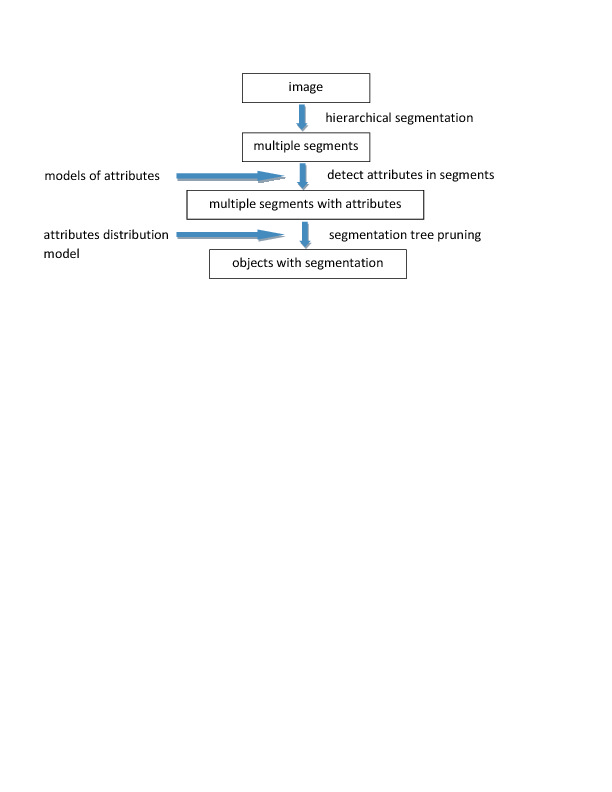
\includegraphics[width=0.80\textwidth]{flowchart.eps}
%\caption{Flow chart of testing phase of our algorithm}
%\label{fig:flow}
%\end{figure}
%
%Figure \ref{fig:flow} shows the basic elements of the testing phase of our algorithm.  
%We begin by hierarchically segmenting the image, retaining the hierarchy of the
%segmentation.  Each segment, or region, is then assigned attributes using the algorithm
%found in \cite{farhadi09}.  We will use the code for this algorithm that is 
%provided by the authors.  
%
%Once we have attributes assigned to each region we set up
%the CRF.  The energy function will look something like this:
%
%\begin{equation}
%\psi(\mb{m}) = \sum_i{\left(\phi(I|m_i)+ \sum_j{f^{\mathsf{pair}}(m_i,m_j,I)} \right)}
%\end{equation}
%
%where
%
%\begin{equation}
%\phi(I|m_i) = f^{\mathsf{relloc}}(S_i, c_i, I) + f^{\mathsf{app}}(S_i, c_i, I)
%\end{equation}
%
%$f^{\mathsf{relloc}}(S_i, c_i, I)$ and $f^{\mathsf{app}}(S_i, c_i, I)$ are defined much in 
%the same spirit as they are in \cite{gould08}.  The relative location feature 
%function requires relative location probability maps which we may build by hand
%or learn (see Tasks section below).  The features will be built from the probability
%maps using a voting scheme as in \cite{gould08}.
%
%We are still unsure what the smoothness function 
%$f^{\mathsf{pair}}(m_i,m_j,I)}$ will look like.  We may learn pairwise attribute
%affinity weights or simply determine a weight based on how many car attributes
%the two regions $S_i$ and $S_j$ have.
%
%As we've chosen to do a binary segmentation (figure, ground) we can use a min-cut-based
%algorithm \cite{boykov01} for the energy minimization of the CRF.  We hope to be able
%to use existing code for this (we can't use the code in \cite{gould08} as they don't
%use min-cut), but have not yet looked carefully.
%
%Once the CRF is in place, we run the energy minimization which gives us the
%segmentation with the estimated highest posterior (if we understand it
%correctly).

%-------------------------------------------------------------------------------
% experimental results
%-------------------------------------------------------------------------------
\section{Experimental results}
\label{sec:results}
Here are some results.

%-------------------------------------------------------------------------------
% conclusions and future work
%-------------------------------------------------------------------------------
\section{Conclusions and future work}
\label{sec:conclusions}
Highly dependent on attribute selection and discriminatory ability of attributes.

%-------------------------------------------------------------------------------
% bibliography
%-------------------------------------------------------------------------------
{\small
%\bibliographystyle{plain}
\bibliographystyle{ieee}
\bibliography{refs}
}

\end{document}
